\documentclass[12pt]{article}
\usepackage[margin=1in]{geometry}
\usepackage{amsmath}
\usepackage{booktabs}
\usepackage{esvect}
\usepackage{float}
\usepackage{graphicx}

\begin{document}
CS7357 HW2, Noah Gardner, 000843905\newline

\section{Assignment 2}
\begin{enumerate}
      \item \textbf{[Points 10]} We learned two linear model - linear regression
            and logistic regression. Compare both methods. Can we use linear
            regression model to detect person face in an image? Describe your
            rationale behind it.

            \textbf{Answer:}
            Linear regression is a linear model that is used to model a linear
            relationship - as an input variable is related to an output variable.
            Logisitic regressions is a linear model that is used to model a binary
            output - for example, given an input variable, the output variable is
            either true or false.

            For detected a face in an image, it might not make sense to use a
            linear model, unless we are trying to count the number of faces in the
            image. Instead, we can use a logistic regression model to output
            'contains a face' or 'does not contain a face' based on the input
            image.

      \item \textbf{[Points 15]} In logistic regression classifier, we are fitting
            a s-shape curve to fit the data. We are given 10 sample points with
            corresponding probabilities as follows, 0.34, 0.21, 0.54, 0.45, 0.60,
            0.70, 0.80, 0.95, 0.99.

            \begin{enumerate}
                  \item \textbf{[Points 7]} What is log odds? Compute log odds
                        values for those given data points.

                        \textbf{Answer:}
                        Odds is a ratio of the probability of success to the
                        probability of failure. Log odds is the logarithm of the
                        odds.

                        \begin{table}[h]
                              \centering
                              \begin{tabular}{c|c|c}
                                    \textbf{Probabilities} & \textbf{Odds} & \textbf{Log Odds} \\
                                    $0.34$                 & $0.515$       & $-0.663$          \\
                                    $0.21$                 & $0.266$       & $-1.325$          \\
                                    $0.54$                 & $1.174$       & $0.16$            \\
                                    $0.45$                 & $0.818$       & $-0.201$          \\
                                    $0.6$                  & $1.5$         & $0.405$           \\
                                    $0.7$                  & $2.333$       & $0.847$           \\
                                    $0.8$                  & $4.0$         & $1.386$           \\
                                    $0.95$                 & $19.0$        & $2.944$           \\
                                    $0.99$                 & $99.0$        & $4.595$           \\
                              \end{tabular}
                        \end{table}
                  \item \textbf{[Points 8]} Compute log likelihood for this given
                        data points.

                        \textbf{Answer:}
                        Log likelihood is the sum of the log odds for each data
                        point.

                        Log likelihood is: $8.15$
            \end{enumerate}

      \item \textbf{[Points 15]} We know logistic regression is a binary
            classifier. Can we use it for multiclass classification? Provide
            detail rationale behind your answer and include any drawback of your
            proposed approaches.

            \textbf{Answer:}
            Since logistic regression is a binary classifier, we can use it for
            multiclass classification with some considerations. First, we might
            consider a series of models which classifies the input as 'A' or 'Not
            A'. If the input is classified as 'Not A', then we can move to the
            next model, which classifies the input as 'B' or 'Not B'. A problem
            with this kind of approach is that the accuracy can be low.

            Another approach is to compare each class to each other class. We
            might have models such as 'A' or 'B', and 'A' or 'C'. A problem with
            this kind of approach is that it can be slow.

      \item \textbf{[Points 10]} SoftMax is a multiclass classifier, and it
            converts logits to probabilities. We are given logit values 3.5, 6.1,
            -2.9, -1.2 for 4 classes “bus”, “truck”, “car”, “van”, respectively.
            Compute the probability of those given logits and classify it.

            \textbf{Answer:}
            \begin{equation}
                  probability = \frac{e^{logit}}{1+e^{logit}}
            \end{equation}

            Output probabilities are: $[0.971, 0.998, 0.052, 0.231]$

            The classifier classifies the input as 'truck'.

      \item \textbf{[Points 25]} We are designing a 2-layer feedforward neural
            network. Our input features are 3-dimensional. The first hidden layer
            has 5 neurons with sigmoid activation function. Final layer contains
            two neurons with Relu activation function. Assume that given inputs
            are $x_1, x_2, x_3$ and hidden layer weights are $w_{ij}^{l}$, where
            $l \in {1, 2}$ is the layer number and $i \in {1,2,3}$ is the number
            of inputs. $j \in {1,2,3,4,5}$ indicates the number of neurons.
            $b_{j}^{j}$ indicates bias for corresponding layers and neurons. For
            any inconsistency with the notation given, you can modify it and
            mentioned the notation scheme in your answer.

            \begin{enumerate}
                  \item \textbf{[Points 10]} Draw a complete diagram of this feed
                        forward neural network showing all individual weights,
                        biases.

                        \textbf{Answer:}

                        \begin{figure}[h]
                              \centering
                              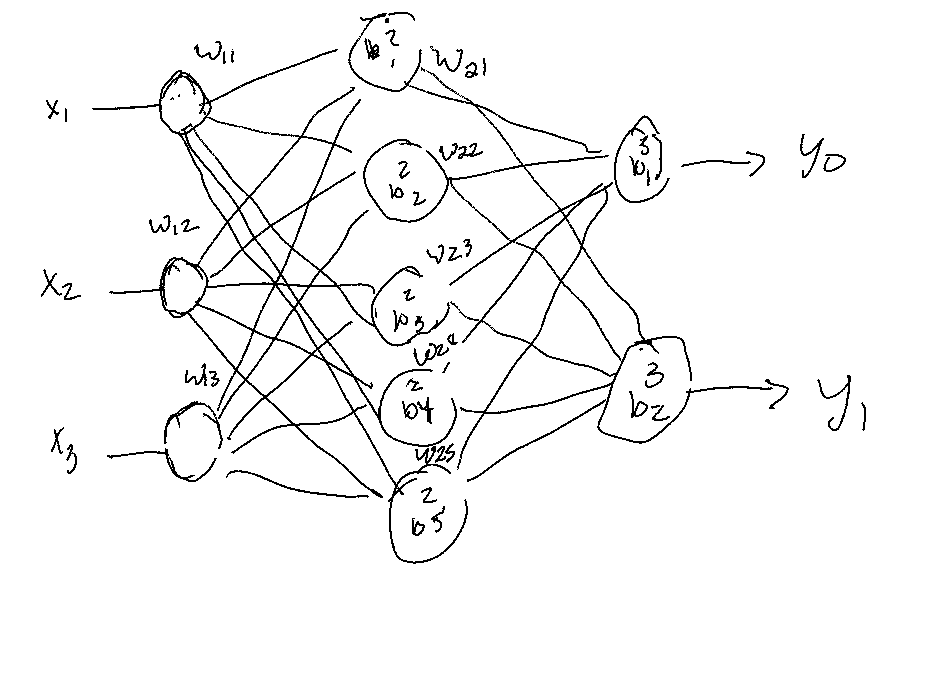
\includegraphics[width=0.8\textwidth]{assets/hw2/neuralnet.png}
                              \caption{Feedforward Neural Network}
                        \end{figure}

                  \item \textbf{[Points 10]} Show forward computation for this given
                        input $x_1, x_2, x_3$. Show detailed equations for each
                        computing unit (neuron) for each layer.

                        \textbf{Answer:}

                        Neurons in the second layer:
                        \begin{equation}
                              z_{1j} = w_{1j}x_{j}
                        \end{equation}

                        Neurons in the second layer:
                        \begin{equation}
                              z_{2j} = sigmoid(w_{11}x_1 + w_{12}x_2 + w_{13}x_3 + b_{j}^{1})
                        \end{equation}

                        Neurons in the third layer:
                        \begin{equation}
                              z_{3j} = relu(w_{21}z_{11} + w_{22}z_{12} + w_{23}z_{13} + w_{24}z_{14} + w_{25}z_{15} + b_{j}^{2})
                        \end{equation}

                        Where $sigmoid$ is the sigmoid function:
                        \begin{equation}
                              sigmoid(z) = \frac{1}{1+e^{-z}}
                        \end{equation}

                        Where $relu$ is the rectified linear unit function:
                        \begin{equation}
                              relu(z) = max(0, z)
                        \end{equation}
            \end{enumerate}
\end{enumerate}
\end{document}